\documentclass[11pt]{article}
\usepackage[utf8]{inputenc}
\usepackage[T2A]{fontenc}
\usepackage[russian]{babel}
\usepackage{amsmath,amssymb}
\usepackage{graphicx}
\usepackage{hyperref}

\title{MCIPS: Maximized-Center Inscribed Parallelepiped Search для MILP}
\author{черновик}
\date{}

\begin{document}
\maketitle

\begin{abstract}
Короткий отчёт-черновик по эвристике MCIPS (Maximized-Center Inscribed
Parallelepiped Search) построения допустимых решений MILP. В допустимую область
LP-релаксации вписывается тело простой формы с максимизированным вдоль $c$
центром, целочисленная вершина берётся как кандидат. Сравниваем два базиса
вписываемого тела: axis-aligned коробку ($B=I$) и параллелепипед с аффинным
базисом. Показываем, что на анизотропной допустимой области параллелепипед
вписывается там, где куб уже несовместен.
\end{abstract}

\section{Постановка}

Рассматривается задача
\begin{equation}
\max\; c^\top x \quad \text{s.t.} \quad A x \le b,\; l \le x \le u,\;
x_i \in \mathbb{Z}\; (i \in I).
\end{equation}
Идея эвристики: вписать в допустимую область широкую область простой формы,
сдвинуть её центр вдоль $c$ и взять целочисленный угол как кандидата.

\section{Кубовая область}

Коробка $x \in [l, u]$. Условие допустимости всех вершин записывается через
опорную функцию: для каждой строки $a_k$
\begin{equation}
\sum_i \big( a_{ki} \ge 0 \,?\, a_{ki} u_i : a_{ki} l_i \big) \le b_k .
\end{equation}
Для целочисленных осей требуем $u_i - l_i \ge \tau$. Цель $\max c^\top(l+u)$.
Это линейная программа с $2n$ переменными.

\section{Параллелепипед}

Пусть базис $B$ фиксирован, область
\begin{equation}
P = \{\, \mathrm{center} + B t : t \in [-e, e] \,\}.
\end{equation}
Так как $B$ фиксирован, $a_k^\top B_i$ - константы, и допустимость вершин
остаётся линейной:
\begin{equation}
a_k^\top \mathrm{center} + \sum_i |a_k^\top B_i|\, e_i \le b_k .
\end{equation}
При $B = I$ получаем в точности кубовый случай.

\section{Наблюдение}

В тонкой наклонной полосе требуемую ширину $\tau$ по целочисленной оси дешевле
набрать вдоль полосы. Куб вынужден набирать её по осям координат и при большом
$\tau$ становится несовместным; параллелепипед, повёрнутый под наклон, всё ещё
вписывается (рис.~\ref{fig:cmp}).

\begin{figure}[h]
\centering
% 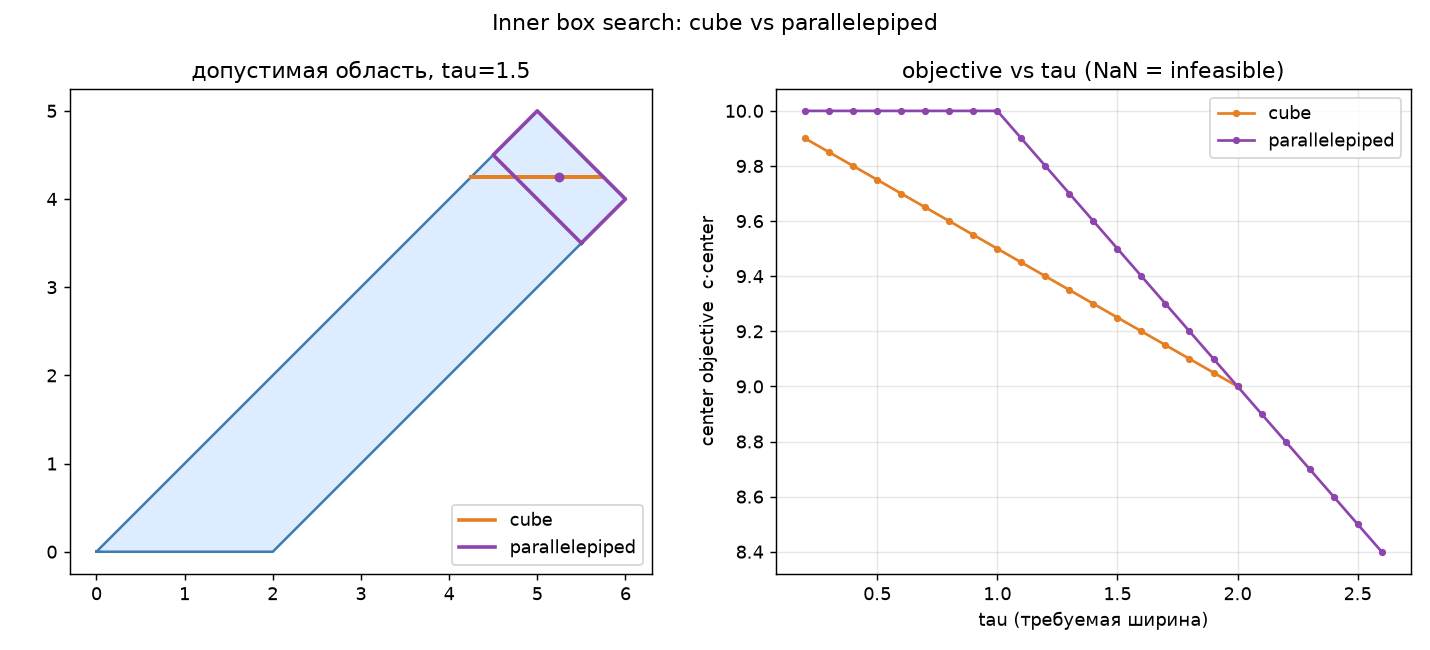
\includegraphics[width=0.9\textwidth]{../docs/figures/cube_vs_parallelepiped.png}
\caption{Слева: вписанные куб и параллелепипед. Справа: $c^\top\mathrm{center}$
как функция $\tau$; куб уходит в infeasible раньше.}
\label{fig:cmp}
\end{figure}

\section{Ограничения}

Базис $B$ задаётся вручную, автоматического выбора нет. Кандидат - эвристика без
гарантии оптимальности MILP. Это учебный прототип, не production-солвер.

\end{document}
